\documentclass{beamer}
\usetheme{Singapore}

\usepackage{verbatim}
\usepackage{url}
\usepackage{epic}
\usepackage{tikz}
\usetikzlibrary{through,calc,intersections}
\usetikzlibrary{arrows.meta,shapes.geometric}
\tikzset{>=stealth}

\newcommand*{\p}[1]{\texttt{#1}}


\title{Ramsey Theory and SAT Solving}
\author{Moti Ben-Ari\\\url{https://www.weizmann.ac.il/sci-tea/benari}}
\institute{Department of Science Teaching\\
Weizmann Institute of Science}
\date{}

\begin{document}

\frame{\titlepage}

%%%%%%%%%%%%%%%%%%%%%%%%%%%%%%%%%%%%%%%%%%%%%%%%%%%%%%

\begin{frame}
\frametitle{Two-Color $K_5$ Without Monochromatic Triangles}

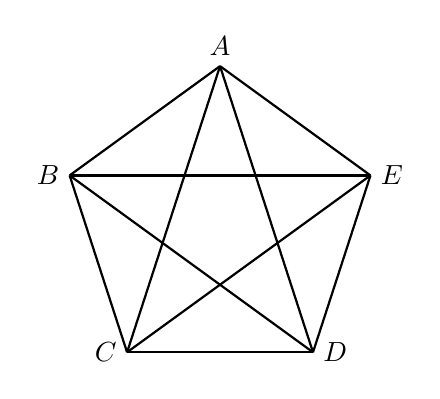
\begin{tikzpicture}
\node (pentagon) [minimum size=4cm,regular polygon,regular polygon sides=5] at (0,0) {};
\draw[thick]  (pentagon.corner 1) node[black,above] {$A$} -- (pentagon.corner 2);
\draw[thick]  (pentagon.corner 2) node[black,left] {$B$} -- (pentagon.corner 3);
\draw[thick]  (pentagon.corner 3) node[black,left] {$C$} -- (pentagon.corner 4);
\draw[thick]  (pentagon.corner 4) node[black,right] {$D$} -- (pentagon.corner 5);
\draw[thick]  (pentagon.corner 5) node[black,right] {$E$} -- (pentagon.corner 1);
\draw[thick] (pentagon.corner 1) -- (pentagon.corner 3);
\draw[thick] (pentagon.corner 1) -- (pentagon.corner 4);
\draw[thick] (pentagon.corner 2) -- (pentagon.corner 4);
\draw[thick] (pentagon.corner 2) -- (pentagon.corner 5);
\draw[thick] (pentagon.corner 3) -- (pentagon.corner 5);
\end{tikzpicture}
\pause
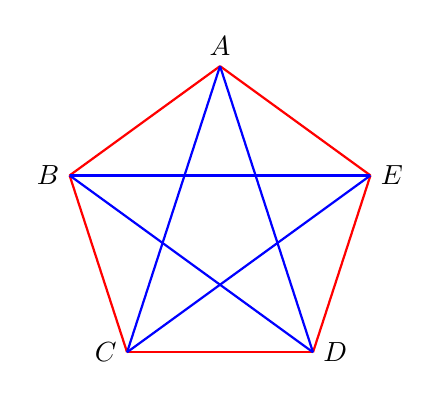
\begin{tikzpicture}
\node (pentagon) [minimum size=4cm,regular polygon,regular polygon sides=5] at (0,0) {};
\draw[red,thick]  (pentagon.corner 1) node[black,above] {$A$} -- (pentagon.corner 2);
\draw[red,thick]  (pentagon.corner 2) node[black,left] {$B$} -- (pentagon.corner 3);
\draw[red,thick]  (pentagon.corner 3) node[black,left] {$C$} -- (pentagon.corner 4);
\draw[red,thick]  (pentagon.corner 4) node[black,right] {$D$} -- (pentagon.corner 5);
\draw[red,thick]  (pentagon.corner 5) node[black,right] {$E$} -- (pentagon.corner 1);
\draw[blue,thick] (pentagon.corner 1) -- (pentagon.corner 3);
\draw[blue,thick] (pentagon.corner 1) -- (pentagon.corner 4);
\draw[blue,thick] (pentagon.corner 2) -- (pentagon.corner 4);
\draw[blue,thick] (pentagon.corner 2) -- (pentagon.corner 5);
\draw[blue,thick] (pentagon.corner 3) -- (pentagon.corner 5);
\end{tikzpicture}

\end{frame}

%%%%%%%%%%%%%%%%%%%%%%%%%%%%%%%%%%%%%%%%%%%%%%%%%%%%%%


\begin{frame}
\frametitle{Two-Color $K_6$ Without Monochromatic Triangles}
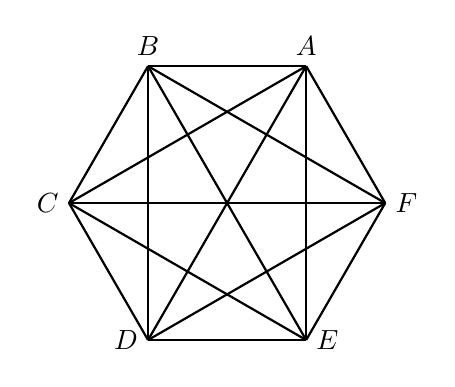
\begin{tikzpicture}
\node (hexagon) [minimum size=4cm,regular polygon,regular polygon sides=6] at (0,0) {};
\draw[thick]  (hexagon.corner 1) node[black,above] {$A$} -- (hexagon.corner 2);
\draw[thick]  (hexagon.corner 2) node[black,above] {$B$} -- (hexagon.corner 3);
\draw[thick]  (hexagon.corner 3) node[black,left] {$C$} -- (hexagon.corner 4);
\draw[thick]  (hexagon.corner 4) node[black,left] {$D$} -- (hexagon.corner 5);
\draw[thick]  (hexagon.corner 5) node[black,right] {$E$} -- (hexagon.corner 6);
\draw[thick]  (hexagon.corner 6) node[black,right] {$F$} -- (hexagon.corner 1);
\draw[thick] (hexagon.corner 1) -- (hexagon.corner 3);
\draw[thick] (hexagon.corner 1) -- (hexagon.corner 4);
\draw[thick] (hexagon.corner 1) -- (hexagon.corner 5);
\draw[thick] (hexagon.corner 2) -- (hexagon.corner 4);
\draw[thick] (hexagon.corner 2) -- (hexagon.corner 5);
\draw[thick] (hexagon.corner 2) -- (hexagon.corner 6);
\draw[thick] (hexagon.corner 3) -- (hexagon.corner 5);
\draw[thick] (hexagon.corner 3) -- (hexagon.corner 6);
\draw[thick] (hexagon.corner 4) -- (hexagon.corner 6);
\end{tikzpicture}
\pause
\hfill
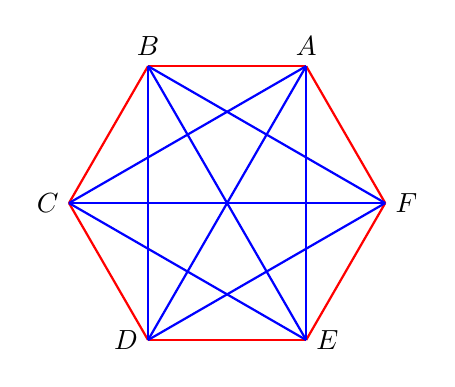
\begin{tikzpicture}
\node (hexagon) [minimum size=4cm,regular polygon,regular polygon sides=6] at (0,0) {};
\draw[red,thick]  (hexagon.corner 1) node[black,above] {$A$} -- (hexagon.corner 2);
\draw[red,thick]  (hexagon.corner 2) node[black,above] {$B$} -- (hexagon.corner 3);
\draw[red,thick]  (hexagon.corner 3) node[black,left] {$C$} -- (hexagon.corner 4);
\draw[red,thick]  (hexagon.corner 4) node[black,left] {$D$} -- (hexagon.corner 5);
\draw[red,thick]  (hexagon.corner 5) node[black,right] {$E$} -- (hexagon.corner 6);
\draw[red,thick]  (hexagon.corner 6) node[black,right] {$F$} -- (hexagon.corner 1);
\draw[thick,blue] (hexagon.corner 1) -- (hexagon.corner 3);
\draw[thick,blue] (hexagon.corner 1) -- (hexagon.corner 4);
\draw[thick,blue] (hexagon.corner 1) -- (hexagon.corner 5);
\draw[thick,blue] (hexagon.corner 2) -- (hexagon.corner 4);
\draw[thick,blue] (hexagon.corner 2) -- (hexagon.corner 5);
\draw[thick,blue] (hexagon.corner 2) -- (hexagon.corner 6);
\draw[thick,blue] (hexagon.corner 3) -- (hexagon.corner 5);
\draw[thick,blue] (hexagon.corner 3) -- (hexagon.corner 6);
\draw[thick,blue] (hexagon.corner 4) -- (hexagon.corner 6);
\end{tikzpicture}
\end{frame}

%%%%%%%%%%%%%%%%%%%%%%%%%%%%%%%%%%%%%%%%%%%%%%%%%%%%%%

\begin{frame}
\frametitle{Two-Colored $K_6$ Must Have Monochromatic Triangles}

\begin{tikzpicture}
\node (hexagon) [minimum size=4cm,regular polygon,regular polygon sides=6] at (0,0) {};
\draw[red]  (hexagon.corner 1) node[black,above] {$A$} -- (hexagon.corner 2) node[black,above] {$B$};
\draw[blue,dashed]  (hexagon.corner 1) -- (hexagon.corner 6) node[black,right] {$F$};
\draw[red] (hexagon.corner 1) -- (hexagon.corner 3) node[black,below] {$C$};
\draw[blue,dashed] (hexagon.corner 1) -- (hexagon.corner 4) node[black,right] {$D$};
\draw[red] (hexagon.corner 1) -- (hexagon.corner 5) node[black,right] {$E$};
\end{tikzpicture}
\hspace{2em}
\pause
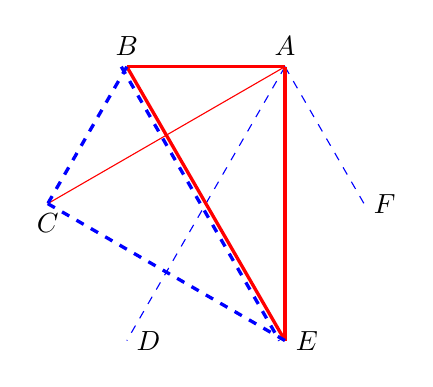
\begin{tikzpicture}
\node (hexagon) [minimum size=4cm,regular polygon,regular polygon sides=6] at (0,0) {};
\draw[very thick,red]  (hexagon.corner 1) node[black,above] {$A$} -- (hexagon.corner 2) node[black,above] {$B$};
\draw[blue,dashed]  (hexagon.corner 1) -- (hexagon.corner 6) node[black,right] {$F$};
\draw[red] (hexagon.corner 1) -- (hexagon.corner 3) node[black,below] {$C$};
\draw[blue,dashed] (hexagon.corner 1) -- (hexagon.corner 4) node[black,right] {$D$};
\draw[very thick,red] (hexagon.corner 1) -- (hexagon.corner 5) node[black,right] {$E$};
\draw[very thick,red] (hexagon.corner 2) -- (hexagon.corner 5);
\draw[very thick,blue,dashed] (hexagon.corner 2) -- (hexagon.corner 3);
\draw[very thick,blue,dashed] ($(hexagon.corner 2)+(-2pt,0)$) -- ($(hexagon.corner 5)+(-2pt,0)$);
\draw[very thick,blue,dashed] (hexagon.corner 5) -- (hexagon.corner 3);
\end{tikzpicture}
\end{frame}

%%%%%%%%%%%%%%%%%%%%%%%%%%%%%%%%%%%%%%%%%%%%%%%%%%%%%%

\begin{frame}
\frametitle{Ramsey's Theorem}
\textbf{Definition:}
$R(k)$, the \emph{Ramsey number} for $k$, is the smallest number $n$ such that in \emph{any} coloring of $K_{n}$, the complete graph on $n$ vertices, with two colors there is a monochromatic complete subgraph $K_k$.

\bigskip

\textbf{Theorem:} For all $k$ the Ramsey number $R(k)$ exists.
\pause
\[
\begin{array}{r|r}
\hline
k & R(k)\\\hline
3 & 6\\
4 & 18\\
5 & 43\text{--}48\\
6 & 102\text{--}165\\
7 & 205\text{--}540\\
8 & 282\text{--}1870
\end{array}
\]
\end{frame}

%%%%%%%%%%%%%%%%%%%%%%%%%%%%%%%%%%%%%%%%%%%%%%%%%%%%%%%%%%

\begin{frame}
\frametitle{Schur Triples}

\textbf{Definition:}
Given \emph{any} decomposition of the set of positive integers:
\[
S(n)=\{1,\ldots,n\}
\]
into two disjoint subsets $S_1,S_2$, do there exist $\{a,b,c\}\subseteq S_1$ or $\{a,b,c\}\subseteq S_2$ (or both) such that $a\!<\!b\!<\!c$ and $a+b=c$? If so, the set $\{a,b,c\}$ is called a \emph{Schur triple}.

\pause

\[
S_1 = \{1,2,3,4,5\},\; S_2 = \{6,7,8\}
\]

\pause

\[
S'_1 = \{1,2,4,7,8\},\; S'_2 = \{3,5\}
\]
\end{frame}

\begin{frame}
\frametitle{Schur Triples for $n=9$}
\[
\begin{array}{l@{\hspace{2em}}l}
S_1&S_2\\\hline
1,3 & \\\hline
1,3 & 2\\\hline
1,3 & 2,4\\\hline
1,3,6 & 2,4\\\hline
1,3,6 & 2,4,7\\\hline
1,3,6,9 & 2,4,7\\\hline
1,3,6,9 & 2,4,7,9
\end{array}
\]

\end{frame}

\begin{frame}
\frametitle{Schur's Theorem}
\textbf{Theorem:}
For every $k\geq 2$ there is a smallest $n$ such that in any disjoint decomposition of $S(n)$ into $k$ subsets, at least one of the subsets must contain a Schur triple.
\end{frame}

%%%%%%%%%%%%%%%%%%%%%%%%%%%%%%%%%%%%%%%%%%%%%%%%%%%%%%%%%%

\begin{frame}
\frametitle{Pythagorean Triples}

\textbf{Definition:}
Given \emph{any} decomposition of the set of positive integers:
\[
S(n)=\{1,\ldots,n\}
\]
into two disjoint subsets $S_1,S_2$, do there exist $\{a,b,c\}\subseteq S_1$ or $\{a,b,c\}\subseteq S_2$ (or both) such that $a\!<\!b\!<\!c$ and $a^2+b^2=c^2$? If so, $\{a,b,c\}$ is called a \emph{Pythagorean triple}.

\pause
\[
S_1 = \{4,5,7,9\},\; S_2=\{1,2,3,6,8,10\}\,,
\]

\pause
\[
S_1 = \{4,5,6,7,9\},\; S_2=\{1,2,3,8,10\}\,,
\]
\end{frame}

%%%%%%%%%%%%%%%%%%%%%%%%%%%%%%%%%%%%%%%%%%%%%%%%%%%%%%

\begin{frame}
\frametitle{Pythagorean Triples Theorem}

\textbf{Theorem:}
For all $n\leq 7824$, there is \emph{some} decomposition of $S(n)$ into two disjoint subsets such that both subsets \emph{do not contain} a Pythagorean triple.

\bigskip

\textbf{Theorem:}
For all $n\geq 7825$, in \emph{all} decompositions of $S(n)$ into two disjoint subsets at least one subset \emph{contains} a Pythagorean triple.

\bigskip

Marijn J. H. Heule and Oliver Kullmann. The Science of Brute Force, \textit{Communications of the ACM} 60(8), 2017, 70--79.

\end{frame}

%%%%%%%%%%%%%%%%%%%%%%%%%%%%%%%%%%%%%%%%%%%%%%%%%%%%%%%%%%%

\begin{frame}
\frametitle{Propositional Logic -- Syntax}

A \emph{formula} is composed of \emph{atoms} connected by the propositional operators $\vee$ (\emph{disjunction}), $\wedge$ (\emph{conjunction}), $\neg$ (\emph{negation}).

\smallskip

If $p$ is an atom then $\neg p$ is a \emph{literal}.

\[
(\neg p \wedge q) \vee \neg(r \vee (\neg p \wedge r))
\wedge (r \wedge p \vee (q \vee \neg r))
\]

\pause

\bigskip

A formula is in \emph{conjunctive normal form (CNF)} if and only if it is composed of a conjunction of subformulas each of which is a disjunction of literals.

\[
(\neg p \vee q \vee \neg \,r) \;\wedge\; (\neg p \vee r)
\;\wedge\; (\neg \,r)\;\wedge\;(p \vee q \vee \neg \,r)
\]

\end{frame}

%%%%%%%%%%%%%%%%%%%%%%%%%%%%%%%%%%%%%%%%%%%%%%%%%%%%%%

\begin{frame}
\frametitle{Propositional Logic -- Semantics}

A formula is given an \emph{interpretation} by an assignment of $T$ or $F$ to each atom. Evaluating a formula in an interpretation results in its \emph{truth value} $T$ or $F$. 

\begin{center}
\begin{tabular}{|c|c||c||c||c|}
\hline
$p$ & $q$ &$\neg p$ &$p \wedge q$& $p \vee q$ \\ \hline \hline
$T$ & $T$ & $F$ &$T$ & $T$  \\ \hline
$T$ & $F$ & $F$ &$F$ & $T$ \\ \hline
$F$ & $T$ & $T$ &$F$ & $T$ \\ \hline
$F$ & $F$ & $T$ &$F$ & $F$ \\ \hline
\end{tabular}
\end{center}

\pause

A formula is \emph{satisfiable} if and only if there is an interpretation that makes its truth value $T$. Otherwise, the formula is \emph{unsatisfiable}.

\pause

The following formula is satisfiable for $p=F,q=?,r=F$.
\[
(\neg p \vee q \vee \neg \,r) \;\wedge\; (\neg p \vee r)
\;\wedge\; (\neg \,r)\;\wedge\;(p \vee q \vee \neg \,r)
\]

\end{frame}

%%%%%%%%%%%%%%%%%%%%%%%%%%%%%%%%%%%%%%%%%%%%%%%%%%%%%%

\begin{frame}
\frametitle{The Meaning of $\vee$}

Is this formula true?
\begin{quote}
$(1+1=2) \vee (1+1=3)$
\end{quote}
\pause

\bigskip

Given that this formula is true, what can you say about the two subformulas?
\begin{quote}
$(1+1=2) \vee (1+1=3)$
\end{quote}

\end{frame}

%%%%%%%%%%%%%%%%%%%%%%%%%%%%%%%%%%%%%%%%%%%%%%%%%%%%%%

\begin{frame}
\frametitle{SAT solvers}

\begin{center}
\begin{tabular}
  {|@{\hspace*{1em}}p{0.9\textwidth}@{\hspace*{1em}}|}
  \hline\\
The \emph{SAT problem} is to decide if a given formula in CNF is satisfiable or not.\\\\\hline
\end{tabular} 
\end{center}

\pause

\bigskip

A \emph{SAT solver}\index{SAT solver} is a computer program that can solve the SAT problem.

\pause

\bigskip

Almost certainly there is no efficient algorithm for SAT.

\bigskip

But, ``efficient'' SAT solvers have been developed.

\end{frame}

%%%%%%%%%%%%%%%%%%%%%%%%%%%%%%%%%%%%%%%%%%%%%%%%%%%%%%

\begin{frame}
\frametitle{Encoding the $1..8$ Schur Triples Problem in CNF}

$p_i$ is $T$ iff $i\in S_1$

$p_i$ is $F$ iff $i\in S_2$

\pause 
The following formula is satisfiable if and only if there \textbf{\Large exists} a decomposition with \textbf{\Large no} Schur triples.
\[
\begin{array}{l}
(p_1 \vee p_2 \vee p_3) \;\wedge\; (\neg p_1 \vee \neg p_2 \vee \neg p_3) \;\wedge \\
(p_1 \vee p_3 \vee p_4) \;\wedge\; (\neg p_1 \vee \neg p_3 \vee \neg p_4) \;\wedge \\
(p_1 \vee p_4 \vee p_5) \;\wedge\; (\neg p_1 \vee \neg p_4 \vee \neg p_5) \;\wedge \\
(p_1 \vee p_5 \vee p_6) \;\wedge\; (\neg p_1 \vee \neg p_5 \vee \neg p_6) \;\wedge \\
(p_1 \vee p_6 \vee p_7) \;\wedge\; (\neg p_1 \vee \neg p_6 \vee \neg p_7) \;\wedge \\
(p_1 \vee p_7 \vee p_8) \;\wedge\; (\neg p_1 \vee \neg p_7 \vee \neg p_8) \;\wedge \\
(p_2 \vee p_3 \vee p_5) \;\wedge\; (\neg p_2 \vee \neg p_3 \vee \neg p_5) \;\wedge \\
(p_2 \vee p_4 \vee p_6) \;\wedge\; (\neg p_2 \vee \neg p_4 \vee \neg p_6) \;\wedge \\
(p_2 \vee p_5 \vee p_7) \;\wedge\; (\neg p_2 \vee \neg p_5 \vee \neg p_7) \;\wedge \\
(p_2 \vee p_6 \vee p_8) \;\wedge\; (\neg p_2 \vee \neg p_6 \vee \neg p_8) \;\wedge \\
(p_3 \vee p_4 \vee p_7) \;\wedge\; (\neg p_3 \vee \neg p_4 \vee \neg p_7) \;\wedge \\
(p_3 \vee p_5 \vee p_8) \;\wedge\; (\neg p_3 \vee \neg p_5 \vee \neg p_8)
\end{array}\label{eq.schur2}
\]
\end{frame}

%%%%%%%%%%%%%%%%%%%%%%%%%%%%%%%%%%%%%%%%%%%%%%%%%%%%%%

\begin{frame}
\frametitle{More Logic}

\begin{center}
$\neg(p \wedge q)\;$ if and only if $\; (\neg p \vee \neg q)$ 

\medskip

$\neg(p \vee q) \;$ if and only if $\; (\neg p \wedge \neg q)$

\pause

\bigskip
\bigskip


$1+1=3$ "implies" $1+1=2\;?$

\pause

\bigskip
\bigskip

$p $ "implies" $ q\;$ if and only if $\;\neg p \vee q$


\end{center}
\end{frame}

%%%%%%%%%%%%%%%%%%%%%%%%%%%%%%%%%%%%%%%%%%%%%%%%%%%%%%

\begin{frame}
\frametitle{Result from SAT solver}
The formula is satisfiable with:
\[
\begin{array}{c@{\hspace{8pt}}c@{\hspace{8pt}}c@{\hspace{8pt}}c@{\hspace{8pt}}c@{\hspace{8pt}}c@{\hspace{8pt}}c@{\hspace{8pt}}c}
p_1&p_2&p_3&p_4&p_5&p_6&p_7&p_8\\\hline
F&F&T&F&T&T&T&F
%T&T&F&T&F&F&F&T
\end{array}
\]
The corresponds to 
$S_1=\{1,2,4,8\}$, $S_2=\{3,5,6,7\}$.

\end{frame}

%%%%%%%%%%%%%%%%%%%%%%%%%%%%%%%%%%%%%%%%%%%%%%%%%%%%%%

\begin{frame}
\frametitle{Solving the $1..9$ Schur Triples Problem}

Add the subformulas:
\[
\begin{array}{l}
(p_1 \vee p_8 \vee p_9) \;\wedge\; (\neg p_1 \vee \neg p_8 \vee \neg p_9) \;\wedge \\
(p_2 \vee p_7 \vee p_9) \;\wedge\; (\neg p_2 \vee \neg p_7 \vee \neg p_9) \;\wedge \\
(p_3 \vee p_6 \vee p_9) \;\wedge\; (\neg p_3 \vee \neg p_6 \vee \neg p_9) \;\wedge \\
(p_4 \vee p_5 \vee p_9) \;\wedge\; (\neg p_4 \vee \neg p_5 \vee \neg p_9)
\end{array}
\]

\pause

\bigskip

The formula is unsatisfiable, meaning:

\smallskip

There is \textbf{\Large no} decomposition that has \textbf{\Large no} Schur triple. 

\smallskip

\textbf{\Large Every} decomposition has \textbf{\Large at least one} Schur triple. 
\end{frame}

%%%%%%%%%%%%%%%%%%%%%%%%%%%%%%%%%%%%%%%%%%%%%%%%%%%%%%

\begin{frame}
\frametitle{The DPLL Algorithm}

Loop until satisfying assignment found or unsatisfiable:

\bigskip
\begin{quote}

Choose some atom $p$ in the formula $A$

Assign $T$ or $F$ to $p$ and evaluate $A$.

%
%\medskip
%
%$\qquad T \vee q \vee r \vee s \vee \cdots$ is true.
%
%$\qquad F \wedge (\cdots \vee \cdots) \wedge (\cdots \vee \cdots) \cdots$ is false.
%
\end{quote}

\bigskip

If unsatisfiable, backtrack.


\end{frame}

%%%%%%%%%%%%%%%%%%%%%%%%%%%%%%%%%%%%%%%%%%%%%%%%%%%%%%

\begin{frame}
\frametitle{Unit Propagation}

If $p=T$ then $p \vee q \vee r$ is satisfiable.

If $p=F$ then $p \vee q \vee r$ is satisfiable iff $q \vee r$ is.

\pause

\bigskip

\[
\begin{array}{l}
(p_1 \vee p_2 \vee p_3) \wedge (\neg p_1 \vee \neg p_2 \vee \neg p_3) \:\wedge \\
(p_1 \vee p_3 \vee p_4) \wedge (\neg p_1 \vee \neg p_3 \vee \neg p_4) \:\wedge \\
(p_3 \vee p_4 \vee p_7) \wedge (\neg p_3 \vee \neg p_4 \vee \neg p_7) \:\wedge \\
(p_3 \vee p_5 \vee p_8) \wedge (\neg p_3 \vee \neg p_5 \vee \neg p_8)\,.
\end{array}
\]
Assign $F$ to $p_1$ and $p_2$:

\pause

\bigskip

$p_3$ \textbf{must} be $T$ and $\neg p_3$ \textbf{must} be $F$!!

\bigskip

$(\neg p_4 \vee \neg p_7) \:\wedge\: (\neg p_5 \vee \neg p_8)$

\end{frame}

%%%%%%%%%%%%%%%%%%%%%%%%%%%%%%%%%%%%%%%%%%%%%%%%%%%%%%
%%%%%%%%%%%%%%%%%%%%%%%%%%%%%%%%%%%%%%%%%%%%%%%%%%%%%%

\begin{frame}

\textbf{Theorem:}
For all $n\leq 7824$, there is \emph{some} decomposition of $S(n)$ into two disjoint subsets such that both subsets \emph{do not contain} a Pythagorean triple.

\pause

\bigskip

One minute of computing time.

\pause

\bigskip

\textbf{Theorem:}
For all $n\geq 7825$, in \emph{all} decompositions of $S(n)$ into two disjoint subsets at least one subset \emph{contains} a Pythagorean triple.

\pause

\bigskip

Two days with $800$ cores: $40,000$ hours of computing time.

\pause

\bigskip
Verification:
\begin{itemize}
\item $200$ terabyte log.
\item Short program to verify log.
\item Mathematical proof to verify the program.
\end{itemize}

\end{frame}

%%%%%%%%%%%%%%%%%%%%%%%%%%%%%%%%%%%%%%%%%%%%%%%%%%%%%%

\begin{frame}[fragile]
\frametitle{LearnSAT}
\begin{verbatim}
:- use_module('../src/dpll').
schur8 :-
  dpll(
  [
  [x1,x2,x3], [~x1,~x2,~x3],
  [x1,x3,x4], [~x1,~x3,~x4],
  [x1,x4,x5], [~x1,~x4,~x5],
  [x1,x5,x6], [~x1,~x5,~x6],
  [x1,x6,x7], [~x1,~x6,~x7],
  [x1,x7,x8], [~x1,~x7,~x8],
  [x2,x3,x5], [~x2,~x3,~x5],
  [x2,x4,x6], [~x2,~x4,~x6],
  [x2,x5,x7], [~x2,~x5,~x7],
  [x2,x6,x8], [~x2,~x6,~x8],
  [x3,x4,x7], [~x3,~x4,~x7],
  [x3,x5,x8], [~x3,~x5,~x8]
  ], _).
\end{verbatim}
\end{frame}

%%%%%%%%%%%%%%%%%%%%%%%%%%%%%%%%%%%%%%%%%%%%%%%%%%%%%%

\begin{frame}[fragile]
\frametitle{The Pigeonhole Problem}
Place $n+1$ pigeons into $n$ holes such that each hole contains at most one pigeon.

\pause

\medskip

Solve the problem for 3 pigeons and 2 holes.

\pause

\medskip

Atom \p{pij} is true if and only if pigeon \p{i} is in hole \p{j}.

\pause

\medskip

For two holes and three pigeons, the set of clauses is:

\begin{verbatim}
  [p11, p12],   [p21, p22],   [p31, p32], 
     % Each pigeon in hole 1 or 2 
  [~p11, ~p21], [~p11, ~p31], [~p21, ~p31],
     % No pair is in hole 1
  [~p12, ~p22], [~p12, ~p32], [~p22, ~p32],
     % No pair is in hole 2
\end{verbatim}
\end{frame}

%%%%%%%%%%%%%%%%%%%%%%%%%%%%%%%%%%%%%%%%%%%%%%%%%%%%%%

\begin{frame}[fragile]
\frametitle{Four pigeons and three holes}

Solve the problem for 3 pigeons and 2 holes.

\pause

\medskip

\begin{verbatim}
  [p11, p12, p13], [p21, p22, p23],
  [p31, p32, p33], [p41, p42, p43], 
  % Each pigeon in at least hole

  [~p11, ~p21], [~p11, ~p31], [~p11, ~p41],
  [~p21, ~p31], [~p21, ~p41], [~p31, ~p41],
  [~p12, ~p22], [~p12, ~p32], [~p12, ~p42],
  [~p22, ~p32], [~p22, ~p42], [~p32, ~p42],
  [~p13, ~p23], [~p13, ~p33], [~p13, ~p43],
  [~p23, ~p33], [~p23, ~p43], [~p33, ~p43]
  % Each hole has at most one pigeon
\end{verbatim}
\end{frame}

%%%%%%%%%%%%%%%%%%%%%%%%%%%%%%%%%%%%%%%%%%%%%%%%%%%%%%

\begin{frame}
\frametitle{The Four Queens Problem}
\begin{center}
\unitlength=1.0pt
\begin{picture}(100,100)
\put(0,0){
  \multiputlist(20,0)(20,0){1,2,3,4}
  \multiputlist(0,20)(0,20){4,3,2,1}
}
\put(10,10){
  \put(0,0){\grid(80,80)(20,20)}
  \put( 0, 20){\makebox(20,20){Q}}
  \put(20, 60){\makebox(20,20){Q}}
  \put(40,  0){\makebox(20,20){Q}}
  \put(60, 40){\makebox(20,20){Q}}
}
\end{picture}
\end{center}
\end{frame}

%%%%%%%%%%%%%%%%%%%%%%%%%%%%%%%%%%%%%%%%%%%%%%%%%%%%%%

\begin{frame}
\frametitle{Ramsey's Theorem}

Can $K_5, K_6$ be two-colored without monochromatic triangles?

\bigskip

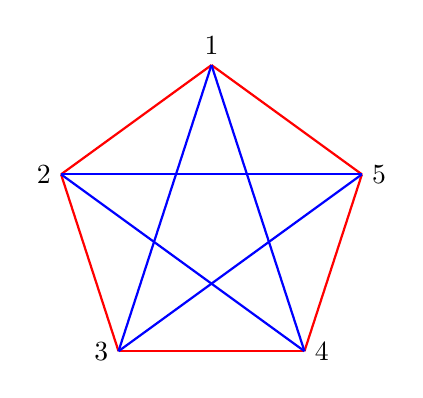
\begin{tikzpicture}
\node (pentagon) [minimum size=4cm,regular polygon,regular polygon sides=5] at (0,0) {};
\draw[red,thick]  (pentagon.corner 1) node[black,above] {$1$} -- (pentagon.corner 2);
\draw[red,thick]  (pentagon.corner 2) node[black,left] {$2$} -- (pentagon.corner 3);
\draw[red,thick]  (pentagon.corner 3) node[black,left] {$3$} -- (pentagon.corner 4);
\draw[red,thick]  (pentagon.corner 4) node[black,right] {$4$} -- (pentagon.corner 5);
\draw[red,thick]  (pentagon.corner 5) node[black,right] {$5$} -- (pentagon.corner 1);
\draw[blue,thick] (pentagon.corner 1) -- (pentagon.corner 3);
\draw[blue,thick] (pentagon.corner 1) -- (pentagon.corner 4);
\draw[blue,thick] (pentagon.corner 2) -- (pentagon.corner 4);
\draw[blue,thick] (pentagon.corner 2) -- (pentagon.corner 5);
\draw[blue,thick] (pentagon.corner 3) -- (pentagon.corner 5);
\end{tikzpicture}
\hfill
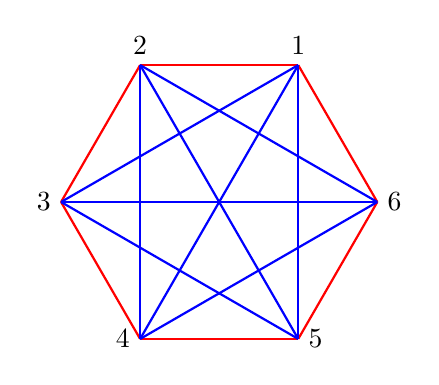
\begin{tikzpicture}
\node (hexagon) [minimum size=4cm,regular polygon,regular polygon sides=6] at (0,0) {};
\draw[red,thick]  (hexagon.corner 1) node[black,above] {$1$} -- (hexagon.corner 2);
\draw[red,thick]  (hexagon.corner 2) node[black,above] {$2$} -- (hexagon.corner 3);
\draw[red,thick]  (hexagon.corner 3) node[black,left] {$3$} -- (hexagon.corner 4);
\draw[red,thick]  (hexagon.corner 4) node[black,left] {$4$} -- (hexagon.corner 5);
\draw[red,thick]  (hexagon.corner 5) node[black,right] {$5$} -- (hexagon.corner 6);
\draw[red,thick]  (hexagon.corner 6) node[black,right] {$6$} -- (hexagon.corner 1);
\draw[thick,blue] (hexagon.corner 1) -- (hexagon.corner 3);
\draw[thick,blue] (hexagon.corner 1) -- (hexagon.corner 4);
\draw[thick,blue] (hexagon.corner 1) -- (hexagon.corner 5);
\draw[thick,blue] (hexagon.corner 2) -- (hexagon.corner 4);
\draw[thick,blue] (hexagon.corner 2) -- (hexagon.corner 5);
\draw[thick,blue] (hexagon.corner 2) -- (hexagon.corner 6);
\draw[thick,blue] (hexagon.corner 3) -- (hexagon.corner 5);
\draw[thick,blue] (hexagon.corner 3) -- (hexagon.corner 6);
\draw[thick,blue] (hexagon.corner 4) -- (hexagon.corner 6);
\end{tikzpicture}
\end{frame}

%%%%%%%%%%%%%%%%%%%%%%%%%%%%%%%%%%%%%%%%%%%%%%%%%%%%%%


\begin{frame}
\frametitle{Graph Coloring Problem}

Decide if one of $k$ colors can be
assigned to each vertex in a graph such that the vertices of a graph do not have the same color.

\bigskip

Show that $K_{2,2}$ is $2$-colorable and that $K_3$ is $3$-colorable.

\bigskip

\begin{center}
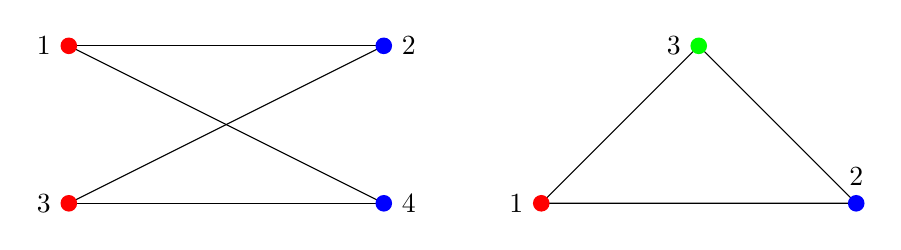
\begin{tikzpicture}
\coordinate (one) at (0,2);
\coordinate (two) at (4,2);
\coordinate (three) at (0,0);
\coordinate (four) at (4,0);
\draw (one) -- (two);
\draw (one) -- (four);
\draw (three) -- (two);
\draw (three) -- (four);
\node[left,xshift=-3pt] at (one) {$1$};
\node[left,xshift=-3pt] at (three) {$3$};
\node[right,xshift=3pt] at (two) {$2$};
\node[right,xshift=3pt] at (four) {$4$};
\fill[red] (one) circle(3pt);
\fill[red] (three) circle(3pt);
\fill[blue] (two) circle(3pt);
\fill[blue] (four) circle(3pt);
\begin{scope}[xshift=6cm]
\coordinate (one) at (0,0);
\coordinate (two) at (4,0);
\coordinate (three) at (2,2);
\draw (one) -- (two) -- (three) -- cycle;
\node[left,xshift=-3pt] at (one) {$1$};
\node[left,xshift=-3pt] at (three) {$3$};
\node[above,yshift=3pt] at (two) {$2$};
\fill[red] (one) circle(3pt);
\fill[green] (three) circle(3pt);
\fill[blue] (two) circle(3pt);
\end{scope}
\end{tikzpicture}
\end{center}

\end{frame}

%%%%%%%%%%%%%%%%%%%%%%%%%%%%%%%%%%%%%%%%%%%%%%%%%%%%%%

\begin{frame}[fragile]
\frametitle{Langford's Problem}
\begin{center}

\begin{tikzpicture}[scale=.9]
\draw[rounded corners,fill=green] (0,0)  
  rectangle +(1.6cm,.8cm);
\draw[rounded corners,fill=red]   (2.2,0)
  rectangle +(1.6cm,.8cm);
\draw[rounded corners,fill=blue]  (4.4,0)
  rectangle +(1.6cm,.8cm);
\draw[rounded corners,fill=red]   (6.6,0)
  rectangle +(1.6cm,.8cm);
\draw[rounded corners,fill=green] (8.8,0)
  rectangle +(1.6cm,.8cm);
\draw[rounded corners,fill=blue]  (11,0)
  rectangle +(1.6cm,.8cm);
\end{tikzpicture}
\end{center}

\bigskip

Langford's problem $L(n)$: Given $1,1,2,2,3,3,\ldots,n,n$, show that they be arranged in a sequence such there are $i$ numbers between the two occurrences of $i$?

\bigskip

Show that $312132$ is a solution for $L(3)$.

\end{frame}

%%%%%%%%%%%%%%%%%%%%%%%%%%%%%%%%%%%%%%%%%%%%%%%%%%%%%%

\begin{frame}
\frametitle{Table for Langford's Problem $n=3$}
\begin{center}
\addtolength{\tabcolsep}{4pt}
\begin{tabular}{|c||c|c|c|c|c|c|}
\hline
&1&2&3&4&5&6\\\hline\hline
1&1&&1&&&\\\hline
2&&1&&1&&\\\hline
3&&&1&&1&\\\hline
4&&&&1&&1\\\hline
5&2&&&2&&\\\hline
6&&2&&&2&\\\hline
7&&&2&&&2\\\hline
8&3&&&&3&\\\hline
9&&3&&&&3\\\hline
\end{tabular}
\end{center}
\end{frame}

%%%%%%%%%%%%%%%%%%%%%%%%%%%%%%%%%%%%%%%%%%%%%%%%%%%%%%

\begin{frame}
\frametitle{Van der Waerden's Problem}

VDW problem: For $k$ colors, what is the smallest $n_k$ such that \emph{any} sequence of $n_k$ colored dots \emph{must} contain an arithmetic progression of $k$ monochromatic dots? 

\bigskip

\begin{center}
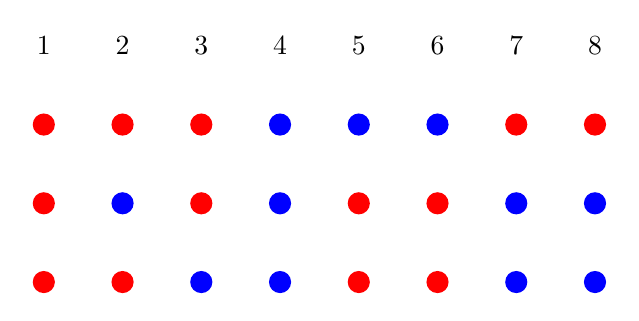
\begin{tikzpicture}
\foreach \x in {1,2,3,4,5,6,7,8} {
  \node at (\x,3) {$\x$};
}
\foreach \x/\col in {1/red,2/red,3/red,4/blue,5/blue,6/blue,7/red,8/red} {
  \fill[\col] (\x,2) circle(4pt);
}
\foreach \x/\col in {1/red,2/blue,3/red,4/blue,5/red,6/red,7/blue,8/blue} {
  \fill[\col] (\x,1) circle(4pt);
}
\foreach \x/\col in {1/red,2/red,3/blue,4/blue,5/red,6/red,7/blue,8/blue} {
  \fill[\col] (\x,0) circle(4pt);
}
\end{tikzpicture}
\end{center}

\pause

\bigskip

Top row: The red dots at positions $(1,2,3)$ form an arithmetic progression as do the blue dots at positions $(4,5,6)$.

\smallskip 

Middle row: The red dots at positions $(1,3,5)$ form an arithmetic progression but the blue dots do not.

\smallskip

Bottom row: No arithmetic progressions.

\end{frame}

%%%%%%%%%%%%%%%%%%%%%%%%%%%%%%%%%%%%%%%%%%%%%%%%%%%%%%

\begin{frame}
\frametitle{Van der Waerden's Problem}

With nine dots \emph{any} coloring \emph{must} contain a sequence of three monochromatic dots that form an arithmetic progression. 

\bigskip

\begin{center}
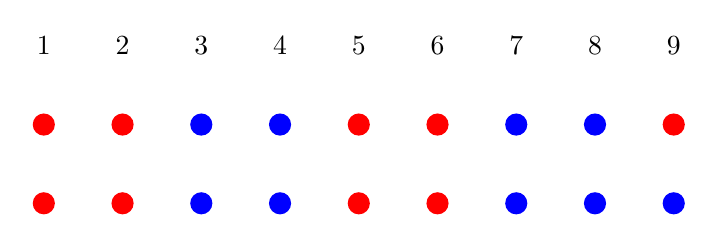
\begin{tikzpicture}
\foreach \x in {1,2,3,4,5,6,7,8,9} {
  \node at (\x,2) {$\x$};
}
\foreach \x/\col in {1/red,2/red,3/blue,4/blue,5/red,6/red,7/blue,8/blue,9/red} {
  \fill[\col] (\x,1) circle(4pt);
}
\foreach \x/\col in {1/red,2/red,3/blue,4/blue,5/red,6/red,7/blue,8/blue,9/blue} {
  \fill[\col] (\x,0) circle(4pt);
}
\end{tikzpicture}
\end{center}
\end{frame}

%%%%%%%%%%%%%%%%%%%%%%%%%%%%%%%%%%%%%%%%%%%%%%%%%%%%%%

\begin{frame}[fragile]
\frametitle{Colored Queens Problem}
Place queens of $k$ colors on an $n\times n$ board such that no color appears more than once in any row, column or diagonal.

\bigskip

Not possible for $k=4, n=4$; possible for $k=5, n=4$.
\begin{center}
\unitlength=1.0pt
\begin{picture}(100,100)
  \put(0,0){\grid(80,80)(20,20)}
  \put( 0, 60){\makebox(20,20){A}}
  \put(20, 60){\makebox(20,20){D}}
  \put(40, 60){\makebox(20,20){C}}
  \put(60, 60){\makebox(20,20){B}}

  \put( 0, 40){\makebox(20,20){B}}
  \put(20, 40){\makebox(20,20){C}}
  \put(40, 40){\makebox(20,20){D}}
  \put(60, 40){\makebox(20,20){A}}

  \put( 0, 20){\makebox(20,20){C}}
  \put(20, 20){\makebox(20,20){B}}
  \put(40, 20){\makebox(20,20){A}}
  \put(60, 20){\makebox(20,20){D}}

  \put( 0, 0){\makebox(20,20){D}}
  \put(20, 0){\makebox(20,20){A}}
  \put(40, 0){\makebox(20,20){B}}
  \put(60, 0){\makebox(20,20){C}}
\end{picture}
\hspace{3em}
\begin{picture}(100,100)
  \put(0,0){\grid(80,80)(20,20)}
  \put( 0, 60){\makebox(20,20){E}}
  \put(20, 60){\makebox(20,20){D}}
  \put(40, 60){\makebox(20,20){C}}
  \put(60, 60){\makebox(20,20){B}}

  \put( 0, 40){\makebox(20,20){C}}
  \put(20, 40){\makebox(20,20){B}}
  \put(40, 40){\makebox(20,20){A}}
  \put(60, 40){\makebox(20,20){E}}

  \put( 0, 20){\makebox(20,20){A}}
  \put(20, 20){\makebox(20,20){E}}
  \put(40, 20){\makebox(20,20){D}}
  \put(60, 20){\makebox(20,20){C}}

  \put( 0, 0){\makebox(20,20){D}}
  \put(20, 0){\makebox(20,20){C}}
  \put(40, 0){\makebox(20,20){B}}
  \put(60, 0){\makebox(20,20){A}}
\end{picture}
\end{center}

Solve for $n=2$, $k=2,3,4$.

\end{frame}


\end{document}
